% !TEX encoding = UTF-8
% !TEX TS-program = pdflatex
% !TEX root = ../tesi.tex

%**************************************************************
\chapter{Definizione del problema}
\label{cap:definizione-problema}
%**************************************************************

\intro{Questo capitolo espone i risultati ottenuti durante i primi tre periodi previsti dal piano di lavoro; al suo interno viene quindi approfondito l'argomento dei problemi di scheduling e viene definito nei dettagli il problema da risolvere durante lo stage. Le informazioni qui presentate sono frutto di uno studio della letteratura di base per i problemi di scheduling: per la sua stesura sono stati consultati i paper ``Introduzione ai problemi di scheduling''\footcite{paper:intro-sched}, ``Modeling staff scheduling problems. A tutorial''\footcite{paper:staff-scheduling}, ``A Hybrid Heuristic Ordering and Variable Neighbourhood Search for the Nurse Rostering Problem''\footcite{paper:nurse-rostering}, ``A Hybrid Scatter Search Heuristic for Personalized Crew Rostering in the Airline Industry''\footcite{paper:crew-rostering}, ``Method for the shift design and personnel task scheduling problem''\footcite{paper:dummy} elencati all'interno della bibliografia.}\\

%**************************************************************
\section{Problemi di scheduling}
Con il termine \textit{scheduling} si intende una vasta classe di problemi decisionali, molto diversi tra loro per
complessità e struttura, in cui riveste importanza il fattore
tempo, visto come risorsa (scarsa) da allocare in modo ottimo a determinate attività; essi quindi ruotano attorno alle modalità di assegnamento all'interno di slot temporali (\ttb, ``Time Table blocks'') di una risorsa (\task) ad un'attività che deve essere effettuata (\items). \\
Una soluzione di un problema di scheduling prende il nome di \textit{schedule}. In termini generali,
una schedule è una descrizione completa dell'utilizzo temporale dei \task\ che devono essere eseguiti dagli \items; nella risoluzione di un problema di schedulazione siamo interessati a schedule ammissibili, cioè che rispettino tutti i vincoli impliciti in qualsiasi problema di scheduling, quali ad esempio che un \task\ non può essere occupato da due \items\ contemporaneamente o che un \items\ non possa essere assegnato a due \task, ma anche altri vincoli determinati dal problema specifico. \\
I vincoli all'interno di un problema di scheduling vengono classificati all'interno di due categorie:
\begin{itemize}
    \item \textbf{Hard constraints:} sono i vincoli inviolabili per il problema, se uno di essi non viene rispettato all'interno di una soluzione, tale soluzione non è ammissibile. Sono vincoli dati dalla natura degli \items\ da schedulare o imposti da fattori esterni, come leggi in merito o regolamenti.
    \item \textbf{Soft constraints:} sono i vincoli che possono essere violati all'interno di una soluzione, producendo ciononostante una soluzione ammissibile. Sono vincoli legati al concetto di \textit{fairness}: produrre una soluzione ``fair'' consiste nel bilanciare il più possibile fra gli \items\ i \task\ o i \ttb\ ritenuti ``impopolari''.
\end{itemize}
Degni di nota all'interno dell'insieme degli \textit{hard constraints} sono i \textit{sequence constraints}, che per ogni \ttb\ \textit{b} definiscono un insieme $\mathcal{T}$\ped{b} che possono seguire \textit{b} per un certo \items. \\ \\
\noindent
Fra tutte le soluzioni ammissibili, chiaramente alcune sono migliori di altre. Il concetto di ``migliore'' viene definito grazie ai \textit{costi} associati ad ogni assegnamento di un \items\ ad un \task\ per un certo \ttb, e a delle \textit{penalità} associate ai \textit{soft constraints}. Ciò che mette insieme costi e penalità è la \textit{funzione obiettivo} il cui valore è un numero, chiamato obiettivo, confrontabile con quello delle altre soluzioni ammissibili per determinare la migliore, ovvero quella che utilizza gli \items\ il più efficientemente possibile.
%**************************************************************
\section{Definizione formale degli elementi generali per i problemi di scheduling}
    \subsection{Dati}
        \paragraph{Item} \textit{s} denota un \items, l'insieme di tutti gli \items\ è indicato con $\mathcal{S}$
        \paragraph{TTB} \textit{b} denota un \ttb, l'insieme di tutti i \ttb\ è indicato con $\mathcal{B}$
        \paragraph{Task} \textit{t} denota un \task, l'insieme di tutti i \task\ è indicato con $\mathcal{T}$
        \paragraph{Costi} \textit{c\ped{sbt}} denota il costo associato all'assegnamento di un \items\ \textit{s} ad un \task\ \textit{t} durante il \ttb\ \textit{b}
        \paragraph{Variabili decisionali} $\mathcal{X}$ denota l'insieme delle variabili decisionali \textit{x\ped{sbt}} t.c.
        \[
        x\ped{sbt} = \begin{cases}
            1,& \text{se l'\items\ \textit{s} è assegnato al \task\ \textit{t} per il \ttb\ \textit{b}}  \\
            0,& \text{altrimenti}
        \end{cases}
        \]
    \subsection{Vincoli}
        \paragraph{Hard} ogni \items\ \textit{s} non può essere assegnato a più di un \task\ \textit{t}, \ttb\ \textit{b} contemporaneamente. \[\sum_{b\in B, t\in T} x\ped{sbt} \le 1, \forall B \forall T \]
        \paragraph{Soft} \textit{c} denota un soft constraint, \textit{f\ped{c}} è la funzione che assegna una penalità a \textit{c}, \textit{f\ped{c}(X)} è la penalità della soluzione \textit{X}.
        \paragraph{Sequence} $\mathcal{T}\ped{b}$ denota l'insieme di \ttb\ che possono essere schedulate dopo la \ttb\ \textit{b}. \[\sum_{b'\in T_b} x\ped{sb't} \ge x\ped{sbt}, \forall b,s,t\]
    \subsection{Obiettivo}
        \paragraph{Costi} il costo \textit{C} di una soluzione \textit{X} è la somma dei costi per ogni assegnamento: \[C=\sum_{s,b,t} x\ped{sbt}*c\ped{sbt}\]
        \paragraph{Fairness} data la misura di popolarità \textit{u\ped{b}} e \textit{u\ped{t}} per ogni \ttb\ \textit{b}, per ogni \task\ \textit{t}; dato \textit{$\alpha$\ped{s}} coefficiente per tenere in conto il carico di lavoro del singolo \items. L'impopolarità della schedule per un \items\ \textit{s} può essere ora definita come:
        
        \[U\ped{s}=\alpha \ped{s} \sum_{b,t}( x\ped{sbt}*u\ped{b} + x\ped{sbt}*u\ped{t})\]
        possiamo stabilire una misura generale di fairness
        \[C\ped{fair}= max U_s - minU_s\]
        \paragraph{Penalità} stabiliamo il costo delle violazioni dei \textit{soft constraints} come:
        \[C\ped{soft}=\sum_{c} f\ped{c}(X)\]
        \paragraph{Funzione obiettivo} per ogni soluzione X:
        \[F(X)= C(X) + C\ped{fair}(X) + C\ped{soft}(X)\]
%**************************************************************
\section{Definizione del problema: scheduling nei casinò}
\subsection{Analisi discorsiva}
All'interno del casinò, l'orizzonte temporale da ricoprire con lo scheduling parte da mezzogiorno e finisce alle sei del mattino dopo. \\Esistono tre categorie di lavoratori: i \textit{dealer}, che possono lavorare nei tavoli; gli \textit{inspector}, che possono lavorare nei pit; i \textit{dealer-inspector} che possono lavorare in entrambe le tipologie di postazione. I dealer hanno un livello da 8 a 1 a seconda della loro esperienza: ogni tavolo richiede un certo livello di esperienza per potervi lavorare. Gli inspector hanno a loro volta un livello da 3 a 1: come succede per i tavoli, anche ogni pit può richiedere un certo livello di inspector.
Inoltre ogni postazione richiede la conoscenza di un determinato gioco; i dealer e gli inspector differiscono per conoscenza di giochi, quindi ci sono postazioni in cui possono o non possono lavorare.\\
Lo scheduler deve fornire uno scheduling in tempi brevi per assicurare un'utilità in decisioni volubili durante l'arco della giornata, poiché la richiesta di copertura dei tavoli dipende dai clienti che arrivano. \\Il turno di un lavoratore è diviso in scaglioni da 20 minuti, il numero totale di ore lavorate in una giornata dipende da ciascun lavoratore; inoltre ci possono essere degli straordinari che vengono decisi dal manager durante la giornata (i lavoratori possono accettarli o meno) fino a 8 ore.\\
Dopo cinque scaglioni consecutivamente lavorati, un lavoratore deve obbligatoriamente avere un turno di pausa, tuttavia è preferibile tenere la media di turni consecutivi intorno ai tre/quattro. Inoltre, dopo ogni pausa il lavoratore non può tornare a lavorare nella stessa postazione dove prestava servizio precedentemente.\\ L'obiettivo è coprire tutte le postazioni aperte con un lavoratore disponibile e bilanciare per quanto possibile lo scheduling in materia di turni consecutivi e postazioni in cui si lavora seduti o in piedi.

\section{Modello per lo scheduling nei casinò}
\subsection{Dati}
\paragraph{Item} sono i lavoratori \textit{s}. \\Per la distizione fra dealer, inspector e dealer-inspector si adottano i parametri \textit{I\ped{s}} e \textit{D\ped{s}} t.c.
\[
I\ped{s} = \begin{cases}
1,& \text{se il lavoratore\ \textit{s} è un inspector}  \\
0,& \text{se il lavoratore\ \textit{s} è un dealer/dealer-inspector}
\end{cases}
\]
\[
D\ped{s} = \begin{cases}
1,& \text{se il lavoratore\ \textit{s} è un dealer}  \\
0,& \text{se il lavoratore\ \textit{s} è un inspector/dealer-inspector}
\end{cases}
\]
Inoltre si definiscono i seguenti parametri:
\[
presente\ped{sb} = \begin{cases}
1,& \text{se il lavoratore\ \textit{s} è può lavorare durante lo scaglione b}  \\
0,& \text{altrimenti}
\end{cases}
\]
\[
straordinari\ped{sb} = \begin{cases}
1,& \text{se il lavoratore\ \textit{s} sta svolgendo straordinari durante lo scaglione b}  \\
0,& \text{altrimenti}
\end{cases}
\]
\[
livello\textunderscore l\ped{s} = \begin{cases}
10-3,& \text{se il lavoratore è un dealer}  \\
3,& \text{se il lavoratore è un dealer-inspector} \\
3-1,& \text{se il lavoratore è un inspector} 
\end{cases}
\]
\[
giochi\textunderscore l\ped{sg} = \begin{cases}
1,& \text{se il gioco g è conosciuto dal lavoratore s}  \\
0,& \text{altrimenti}
\end{cases}
\]
\paragraph{TTB} sono gli scaglioni temporali \textit{b} da 1 a 54. Si definisce il seguente parametro:
\[
popularity\ped{t} = \begin{cases}
1,& \text{se lo scaglione b non è popolare}  \\
0,& \text{altrimenti}
\end{cases}
\]
\paragraph{Task} sono le postazioni da occupare \textit{t}.  Si definiscono i seguenti parametri:
\[
livello\textunderscore p\ped{t} = \begin{cases}
10-3,& \text{se la postazione t è un tavolo}  \\
3-1,& \text{altrimenti} 
\end{cases}
\]
\[
giochi\textunderscore p\ped{tg} = \begin{cases}
1,& \text{se il gioco g è richiesto alla postazione t}  \\
0,& \text{altrimenti}
\end{cases}
\]
\[
popularity\ped{t} = \begin{cases}
1,& \text{la postazione t richiede di stare in piedi}  \\
0,& \text{altrimenti}
\end{cases}
\]
\[
aperto\ped{t} = \begin{cases}
1,& \text{la postazione t è aperta}  \\
0,& \text{altrimenti}
\end{cases}
\]
\[
k = \text{numero di tavoli}
\]
\paragraph{Costi} \textit{c\ped{st}} denota il costo associato all'assegnamento di un lavoratore \textit{s} durante uno scaglione \textit{b} (gli straordinari hanno una maggiorazione dello stipendio)
\paragraph{Variabili decisionali} $x,z \in \mathcal{X}$ t.c.
\[
x\ped{sbt} = \begin{cases}
1,& \text{se il lavoratore \textit{s} è assegnato alla postazione \textit{t} per lo scaglione \textit{b}}  \\
0,& \text{altrimenti}
\end{cases}
\]
\[
z\ped{s} = \text{numero di turni lavorati consecutivamente dal lavoratore s}
\]
\subsection{Vincoli}
\paragraph{Hard}
\begin{itemize}
    \item Lavoratore \textit{s} può fare turno solo se presente in sala e non può fare più di un turno alla volta:
    \[\sum_{t} x\ped{sbt} \le presente\ped{sb}, \forall s,b \]
    \item Tutte le postazioni \textit{t} aperte devono avere qualcuno che ci lavori:
    \[\sum_{s} x\ped{sbt} = aperto\ped{t}, \forall b,t \]
    \item Un inspector non può lavorare in un tavolo:
    \[\sum_{t \le k} I\ped{s}*x\ped{sbt} = 0, \forall s,b \]
    \item Un dealer non può lavorare in un pit:
    \[\sum_{t > k} D\ped{s}*x\ped{sbt} = 0, \forall s,b \]
    \item Ogni postazione t richiede un lavoratore con un livello uguale o più alto al proprio:
    \[x\ped{sbt}*livello\textunderscore l\ped{s} \le livello\textunderscore p\ped{t}, \forall s,b,t \]
    \item Ogni postazione t richiede un lavoratore che conosca il gioco:
    \[x\ped{sbt}*giochi\textunderscore p\ped{tg} = giochi\textunderscore l\ped{st}, \forall s,b,t,g \] 
\end{itemize}
\paragraph{Soft}
\begin{itemize}
    \item I turni dei lavoratori preferibilmente devono essere di tre/quattro scaglioni consecutivi:
    \[z\ped{s} \ge \sum_{j,t}x\ped{sbt}, \forall s \]
    \item Fairness per il numero di scaglioni in piedi/seduti:
    \[fair\ped{s} = \sum_{j,t}x\ped{sbt}*popularity\ped{t}, \forall s \]
\end{itemize}
\paragraph{Sequence} 
\begin{itemize} 
     \item Dopo cinque scaglioni lavorati consecutivamente, uno deve essere di pausa:
    \[\sum_{b = m...m+5} \sum_{t} x\ped{sbt} \le 5, \forall s, m=1...49 \]
    \item Dopo cinque scaglioni lavorati e una pausa, il lavoratore deve cambiare tavolo:
    \[\sum_{b = m...m+6} \sum_{t} x\ped{sbt} \le 5, \forall s, m=1...48 \]
    \item Non possono esserci due pause consecutive:
    \[\sum_{b = m...m+1} \sum_{t} x\ped{sbt} \ge 1, \forall s, m=1...53 \]
\end{itemize}
\subsection{Obiettivo}
\[ min (\sum_{s}(\sum_{b,t}(straordinari\ped{sb}*c\ped{sbt}) + z\ped{s}+fair\ped{s}) \]

\section{Algoritmi euristici di risoluzione per problemi di scheduling}
Nella letteratura è difficile trovare un algoritmo che vada a creare uno scheduling iniziale per i problemi di schedulazione in maniera veloce, i paper si concentrano spesso su metaeuristiche che vadano infatti a migliorare una possibile soluzione iniziale già presente. \\
\\
Nel paper \textit{“A Hybrid Scatter Search Heuristic for Personalized Crew Rostering in the Airline Industry”} sono nominate tre diverse metodologie per trovare uno scheduling iniziale: la prima genera tutte le soluzioni in maniera random andando poi a tenere in considerazione solo le soluzioni ammissibili, la seconda genera le soluzioni euristicamente (ma non viene specificato come), la terza strategia genera invece una parte della soluzione utilizzando un’euristica e la restante parte in maniera randomica. Una volta ottenuta in questo modo una schedule iniziale, viene applicata una Scatter Search (metaeuristica).\\
\\
Basandosi invece sul paper \textit{“A Hybrid Heuristic Ordering and Variable Neighbourhood Search for the Nurse Rostering Problem”}, per creare la schedule iniziale viene utilizzato un algoritmo Greedy.
L’obiettivo è ordinare, tramite una funzione di ordinamento euristica, tutti i turni secondo la difficoltà stimata di assegnazione o quanto è probabile che tale turno causi alta penalità. 
Una volta che i turni sono stati ordinati, sono assegnati in ordine: in questa maniera, i turni più complicati sono assegnati per primi nel processo di costruzione della schedule. Uno alla volta, i turni sono assegnati a tutte le possibili infermiere e si calcola la penalità in cui si incorre compiendo tale assegnazione; il turno è assegnato quindi nella maniera che garantisca la penalità più bassa (le penalità consistono in turni unpopular, tipo turno di notte, al weekend, numero di persone capaci di fare qul lavoro, etc… e consistono in un \textit{weight} assegnato ad ogni turno). Si passa poi a valutare il turno successivo.\\
Una volta ottenuta in questo modo una schedule iniziale, viene applicata una Variable Neighbourhood Search (metaeuristica).
\\ \\
Tenendo conto di queste informazioni, al fine di estendere il framework aziendale con la risoluzione dei problemi di scheduling (con applicazione al problema del casinò) e creare una schedule iniziale ammissibile, ho considerato di:
\begin{itemize}
\item Creare una soluzione random;
\item Utilizzare un algoritmo greedy;
\item Utilizzare in un primo momento un algoritmo greedy, per poi completare la soluzione in maniera randomica.
\end{itemize}
\noindent
L’ipotesi della soluzione random è stata ad un primo impatto scartata in quanto i vincoli di cui tenere conto sono numerosi e molto stringenti, cercare una soluzione random sembra perciò dispersivo e poco efficiente; si è optato quindi per utilizzare un algoritmo greedy ispirato al Nurse Rostering. \\
L’opzione di completare la soluzione in maniera randomica una volta assegnati i turni più complicati è stata tenuta in considerazione, ma non è stata implementata durante il corso dello stage.
\\ \\
Nel dettaglio, l'algoritmo di risoluzione implementato per andare a creare la migliore schedule possibile è stato il seguente:
\begin{enumerate}
\item Per ogni \ttb, per ogni \task, valutare quanti sono gli \items\ disponibili ad essere schedulati. Ordinare quindi per priorità i \task\ da assegnare all'interno del \ttb.
\item Se esiste un \task\ con nessun \items\ disponibile per la schedulazione, è impossibile trovare una soluzione ammissibile. L'algoritmo si interrompe.
\item Vengono valutati tutti i possibili \items\ per il primo \task\ in ordine di priorità. L'\items\ che garantisce il minor obiettivo viene schedulato per il \task\ durante il \ttb. È questa la ``scelta greedy'' dell'algoritmo.
\item Se non ancora tutti i \task\ sono stati schedulati per il \ttb, viene ricalcolata la priorità di assegnamento dei \task\ alla luce dell'assenza di disponibilità dell'ultimo \items\ schedulato. Si ripete dal punto 2.
\item Quando tutti i \task\ del \ttb\ sono stati assegnati ad un \items, si procede con l'assegnare i \task\ del prossimo \ttb, se esiste. Si ripete dal punto 1.
\item Se sono stati assegnati tutti i \task\ dell'ultimo \ttb, si è trovata una soluzione ammissibile.
\end{enumerate}

\begin{figure}[!h]
    \begin{widepage}
        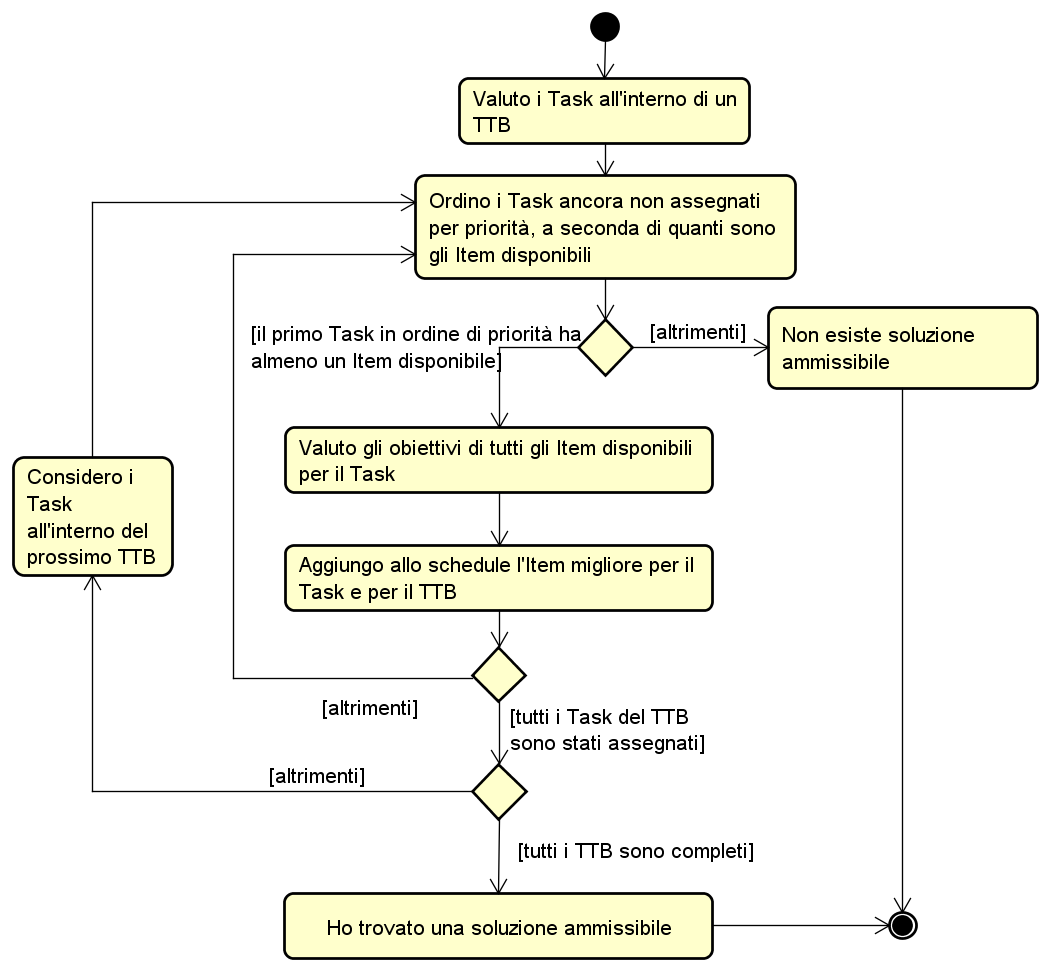
\includegraphics[width=14.9cm,keepaspectratio]{../immagini/algoritmo.png}
        \caption{Diagramma di attività per l'algoritmo greedy di risoluzione per i problemi di scheduling}
    \end{widepage}
\end{figure}
\FloatBarrier
\noindent
Si presenta tuttavia un problema: nel caso in cui gli \items\ non siano abbastanza da coprire tutti i \task\ durante i \ttb, questo algoritmo si blocca e non produce alcuno scheduling. Sapendo che tramite l'euristica si vuole creare uno scheduling iniziale da ottimizzare poi tramite metodi metaeuristici, il non riuscire a produrre uno scheduling iniziale è disturbante. \\
\\
Nel paper \textit{``Method for the shift design and personnel task scheduling problem''}, per arrivare sempre a una soluzione ammissibile viene introdotto un \emph{\gls{dummy}}\glsfirstoccur
, che viene poi eliminato tramite la Neighborhood Search (metaeuristica). \\
\\
L'algoritmo di risoluzione implementato viene quindi lievemente modificato, sostituendo al secondo punto ``Se esiste un \task\ con nessun \items\ disponibile per la schedulazione, il \task\ viene assegnato al Dummy Worker''.
\begin{figure}[!h]
    \begin{widepage}
        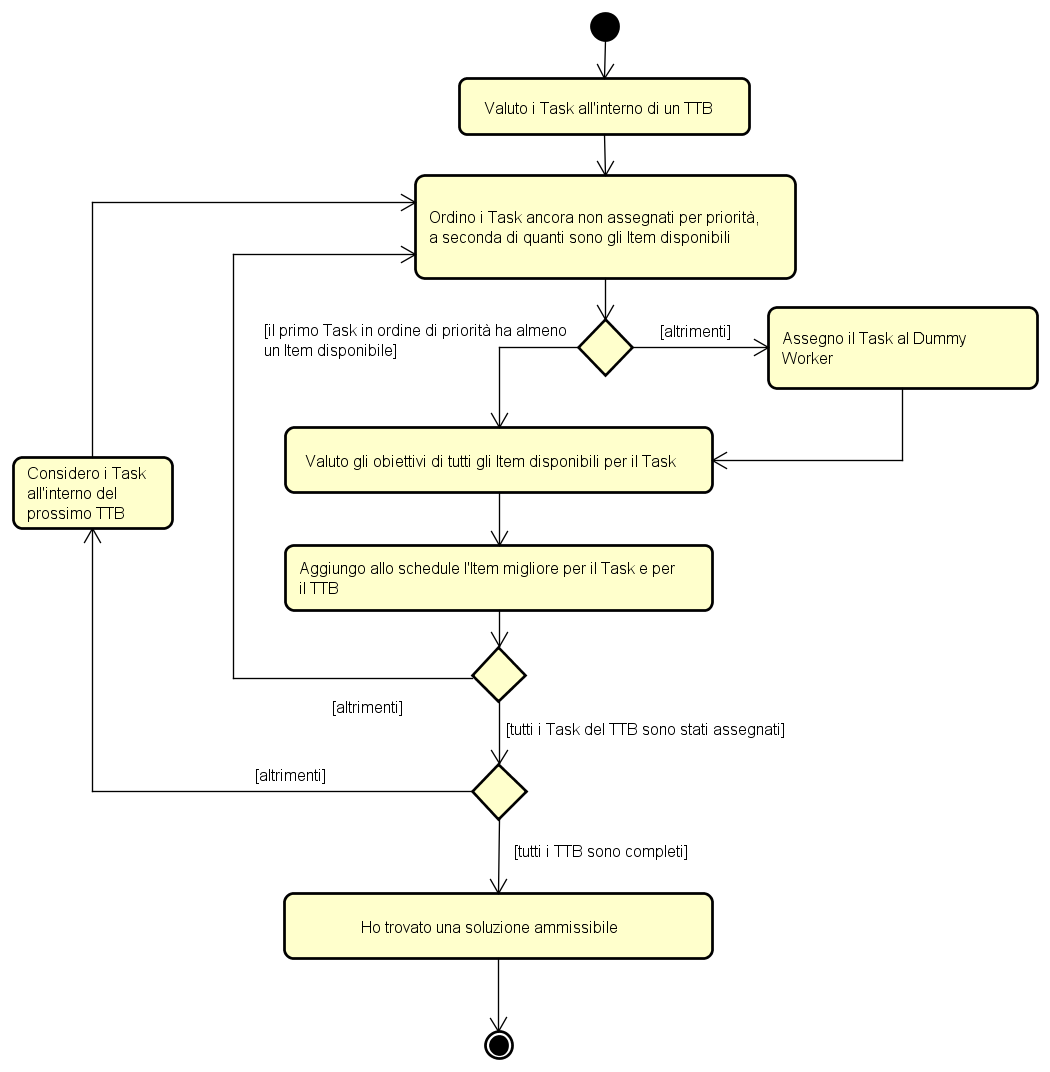
\includegraphics[width=14.9cm,keepaspectratio]{../immagini/algoritmo_dummy.png}
        \caption{Diagramma di attività per l'algoritmo greedy di risoluzione per i problemi di scheduling con aggiunta di Dummy Worker}
    \end{widepage}
\end{figure}